% Options for packages loaded elsewhere
\PassOptionsToPackage{unicode,pdfusetitle}{hyperref}
\PassOptionsToPackage{hyphens}{url}
\PassOptionsToPackage{dvipsnames,svgnames*,x11names*}{xcolor}

\documentclass[10pt,ignorenonframetext]{beamer}
\usepackage{lmodern}
\usepackage{amssymb,amsmath,mathtools,amsthm}
\usepackage[T1]{fontenc}
\usepackage[utf8]{inputenc}
\usepackage{textcomp} % provide euro and other symbols

\usepackage{pgfpages}

% prevent slide breaks in the middle of a paragraph
\widowpenalties 1 10000
\raggedbottom

% redefine part, section, and subsection headers
\raggedbottom
\setbeamertemplate{part page}{
 \centering
 \begin{beamercolorbox}[sep=16pt,center]{part title}
    \usebeamerfont{part title}\insertpart\par
 \end{beamercolorbox}
}
\setbeamertemplate{section page}{
 \centering
 \begin{beamercolorbox}[sep=12pt,center]{part title}
    \usebeamerfont{section title}\insertsection\par
 \end{beamercolorbox}
}
\setbeamertemplate{subsection page}{
 \centering
 \begin{beamercolorbox}[sep=8pt,center]{part title}
    \usebeamerfont{subsection title}\insertsubsection\par
 \end{beamercolorbox}
}

\AtBeginPart{\frame{\partpage}}
\AtBeginSection{\ifbibliography\else\frame{\sectionpage}\fi}
\AtBeginSubsection{\frame{\subsectionpage}}

% beamer configuration
\usecolortheme{dove}
\usefonttheme{professionalfonts}
\usefonttheme{structurebold}
\setbeamertemplate{footline}[frame number]
\setbeamertemplate{caption}[numbered]
\setbeamertemplate{caption label separator}{: }
\setbeamercolor{caption name}{fg=normal text.fg}
\setbeamertemplate{frametitle}{\begin{centering}\insertframetitle\par\end{centering}}
\setbeamertemplate{itemize items}[circle]
\setbeamerfont{frametitle}{size=\large}
\setbeamertemplate{headline}{\vskip5ex}
\beamertemplatenavigationsymbolsempty
%\setlength{\parskip}{1em} % add paragraph spacing

% Use upquote if available, for straight quotes in verbatim environments
\usepackage{upquote}
\usepackage[]{microtype}
\UseMicrotypeSet[protrusion]{basicmath} % disable protrusion for tt fonts

\usepackage{xcolor}
\usepackage{xurl} % add URL line breaks if available
\usepackage{bookmark}
\usepackage{hyperref}
\hypersetup{
  colorlinks=true,
  linkcolor=Maroon,
  filecolor=Maroon,
  citecolor=Blue,
  urlcolor=Blue
}

% tikz and pgfplots stuff
\usepackage{tikz}
\usetikzlibrary{arrows,shapes,positioning,intersections}
\usepackage{pgfplots}
\usepgfplotslibrary{external,colormaps}
\pgfplotsset{width=7cm,compat=1.11}
\tikzexternalize

\urlstyle{same} % disable monospaced font for URLs
\newif\ifbibliography
\setlength{\emergencystretch}{3em} % prevent overfull lines
\setcounter{secnumdepth}{-\maxdimen} % remove section numbering

%\usepackage{subfig}
\usepackage{subcaption}
\usepackage{algorithm,algpseudocode}
\usepackage{booktabs}

\DeclareMathOperator*{\argmax}{arg\,max}
\DeclareMathOperator*{\argmin}{arg\,min}
\DeclareMathOperator{\E}{\text{E}}
\DeclareMathOperator{\var}{var}
\DeclareMathOperator{\cov}{cov}
\DeclareMathOperator{\sign}{sign}
\DeclareMathOperator{\card}{card}
\DeclareMathOperator{\cumsum}{cumsum}
\DeclareMathOperator*{\prox}{prox}
\newcommand{\pkg}[1]{\textsf{#1}}
\renewcommand{\vec}{\vectorsym}
\newcommand{\mat}{\matrixsym}
\newcommand{\du}{\mathrm{d}}

% biblatex
\usepackage[citestyle=authoryear]{biblatex}
\addbibresource{references.bib}

\title{The Strong Screening Rule for SLOPE}
\subtitle{Mathematical Methods of Modern Statistics 2}
%\author{Johan Larsson}
\author[shortname]{\texorpdfstring{\alert{Johan Larsson}}{Johan Larsson}\inst{1} \and Małgorzata Bogdan\inst{1,2} \and Jonas Wallin\inst{1}}
\institute[shortinst]{\inst{1} Department of Statistics, Lund University, \and %
                    \inst{2} Department of Mathematics, University of Wroclaw}
%\institute{Department of Statistics, Lund University}
\date{June 16, 2020}
\titlegraphic{\includegraphics{lu.pdf}}

\begin{document}
\frame[noframenumbering,plain]{\titlepage}

% \hypertarget{first-section}{%
% \section{Setting}\label{first-section}}

\begin{frame}{Sorted L-One Penalized Estimation (SLOPE)}
    The SLOPE ~\autocite{bogdan2015} estimate is 
    \[
    \hat\beta = \argmin_{\beta \in \mathbb{R}^p}\left\{ g(\beta) + J(\beta;\lambda) \right\}
    \]
    where \(J(\beta;\lambda)=\sum_{i=1}^p\lambda_i \lvert \beta \rvert_{(i)}\) is the \alert{sorted \(\ell_1\) norm},
    where
    \[
        \lambda_1 \geq \lambda_2 \geq \cdots \geq \lambda_p \geq 0, \qquad 
        \lvert \beta \rvert_{(1)} \geq \lvert \beta \rvert_{(2)} \geq \cdots \geq \lvert \beta \rvert_{(p)}.
    \]
    \medskip
    \begin{columns}[c]
        \begin{column}{0.45\textwidth}
            Equivalent to an inequality-constrained convex 
            optimization problem
        \end{column}
        \begin{column}{0.45\textwidth}
            \pgfplotsset{width=6cm,height=6cm}
            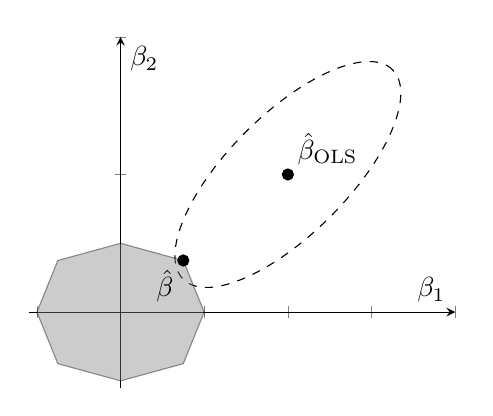
\begin{tikzpicture}
\begin{axis}[
    xlabel = \(\beta_1\),
    ylabel = \(\beta_2\),
    ymin = -1.1,
    ymax = 4,
    xmin = -1.1,
    xmax = 4,
    axis lines = center,
    yticklabels={,,},
    xticklabels={,,}
]

\draw[dashed, rotate around={45:(2,2)}] (2,2) ellipse (1.77 and 0.87);

\addplot[fill = gray, opacity = 0.4]
    coordinates {
    	(-1,0)
    	(-0.75, 0.75)
    	(0,1)
    	(0.75,0.75)
    	(1,0)
    	(0.75,-0.75)
    	(0,-1)
    	(-0.75,-0.75)
    	(-1,0)
    };
\addplot [only marks, mark=*] coordinates {(2,2)};
\node [above right,black] at (2,2) {\(\hat\beta_\text{OLS}\)};

\addplot [only marks, mark=*] coordinates { (0.75,0.75) };
\node [below left] at (0.75,0.75) {$\hat\beta$};
\end{axis}
\end{tikzpicture}   
        \end{column}
    \end{columns}
\end{frame}

\begin{enumerate}\item<1-> A first one,\item<2-> a second one with a bunch of subpoints,\begin{itemize}\item first subpoint. (Only shown from second slide on!).\item<3-> second subpoint added on third slide.\item<4-> third subpoint added on fourth slide.\end{itemize}\item<5-> and a third one.\end{enumerate}
    
\begin{frame}{Motivation for screening rules}
    \begin{columns}
        \begin{column}[t]{0.45\textwidth}
            \begin{itemize}
                \item<1->
                    we are interested in a \alert{path} of
                    penalties \(\lambda^{(1)}, \lambda^{(2)}, \dots, \lambda^{(m)}\),
                    many of which will lead to \alert{sparse}
                    solutions
                \item<2->
                    \alert{basic idea}: what if we could, based on a relatively \alert{cheap} test, determine which
                    predictors will be inactive before fitting the model?
                \item<3->
                    it turns out that we can, using screening rules!
            \end{itemize}
        \end{column}
        \begin{column}[t]{0.45\textwidth}
            \begin{figure}
            \centering
            \includegraphics[width=\linewidth]{figures/slope-path.pdf}
            \caption{SLOPE path with \(n=200\), \(p = 20000\). \(\sigma\) indicates strength of regularization.}
            \end{figure}
        \end{column}
    \end{columns}
\end{frame}

\begin{frame}{Strong screening rule for SLOPE}
    Assume that we have a solution for \(\lambda^{(k-1)}\) and want
    the solution at \(\lambda^{(k)}\).\medskip
    
    Using the optimality condition for the SLOPE problem,
    \[ \textbf{0} \in \nabla g\big(\beta(\lambda^{(k)})\big) + \partial J\big(\beta(\lambda^{(k)});\lambda^{(k)}\big),\]
    where \(\partial J\) is the subgradient, we can determine which predictors will be active at \(\lambda^{(k)}\).

    \pause
    \begin{block}{our contribution}
        approximate \(\nabla g\big(\beta(\lambda^{(k)})\big) \) and use optimality
        criterion (as if \(\nabla g\big(\beta(\lambda^{(k)})\big) \) was known) to discard predictors
    \end{block}
    \pause
    \begin{block}{violations}
        \begin{itemize}
            \item violations---incorrectly discarding predictors---may occur
            \item can always be caught by checking optimality conditions (and refitting if present)
            \item are \alert{so rare} that, in practice, the benefits from using the rule far outweigh the costs it incurs
        \end{itemize}
    \end{block}
\end{frame}

\begin{frame}{Efficiency for real data}
\begin{figure}
\centering
\includegraphics[width=\linewidth]{figures/efficiency-real.pdf}
\caption{Efficiency for real data sets. The dimensions of the predictor matrices
are \(100 \times 9920\) (arcene), \(800\times 88119\) (dorothea), \(6000\times 4955\)
(gisette), and \(38 \times 7129\) (golub).}
\end{figure}
\end{frame}

\begin{frame}{Performance}
\begin{figure}
\centering
\includegraphics[width=\linewidth]{figures/performance.pdf}
\caption{Performance benchmarks for various generalized linear models
with \(X \in \mathbb{R}^{200 \times 20000}\). Predictors are autocorrelated through an
\(\operatorname{AR}(1)\) process with correlation \(\rho\).}
\end{figure}
\end{frame}

\begin{frame}[allowframebreaks]{References}
  \bibliographytrue
  \printbibliography[heading=none]
\end{frame}

\end{document}
